% Provenance (never printed): old premiere S material on the lithosphere and the
% asthenosphere (chemical and mechanical layers, the low-velocity zone, the
% geotherm, isostasy); see sources/book2/PROVENANCE.md. S speeds from
% figdata/grade-11/prem_profiles.py (part upper), the geotherm and the solidus
% from geotherm_solidus.py, the elevations from hypsometry.py (ETOPO1).
% Glacial rebound belongs to g12; lithostatic pressure (term) to g12.
\chapter{Lithosphere and Asthenosphere}\label{ch:g11:lithosphere-asthenosphere}

Nine tenths of an iceberg lie under water: the ice floats because it is a
little less dense than the sea, and it sinks into the water until the water it
pushes aside weighs as much as the whole iceberg. Mountain ranges behave in
much the same way. Under the highest of them the crust is nearly twice as
thick as usual, and most of that extra crust lies hidden underneath, like the ice under
the waterline. But an iceberg floats in a liquid, and the mantle beneath a
mountain range is solid rock. This chapter shows how a solid can behave like a
fluid on which the outer shell of the Earth floats, and what that shell is.
% ledger: usgs:ice-density, karplus:tibet-moho, cm95:crust

\begin{recall}
The Earth has a crust, a mantle and a core (Book 1, grade 6). The \omterm{def:g11:seismic-structure:moho}{Moho}, at the
base of the crust, lies about \qty{41}{km} down under the continents on
average and a few kilometres below the ocean floor; seismic speeds and
densities are known at every depth from a \omterm{def:g11:seismic-structure:reference-model}{reference Earth model}
(\cref{ch:g11:seismic-structure}). The rock gets hotter with depth, by about
25 to \qty{30}{\celsius} per kilometre near the surface (Book 1, grade 6). A
body floating in a liquid pushes aside a weight of liquid equal to its own
weight, and the pressure at the bottom of a column of material is the weight
of the column divided by its area (the physics books).
\end{recall}
% ledger: cm95:crust, usgs:crust-thickness, usgs:gradient-29 (Book 1 rows)

\begin{omfigure}
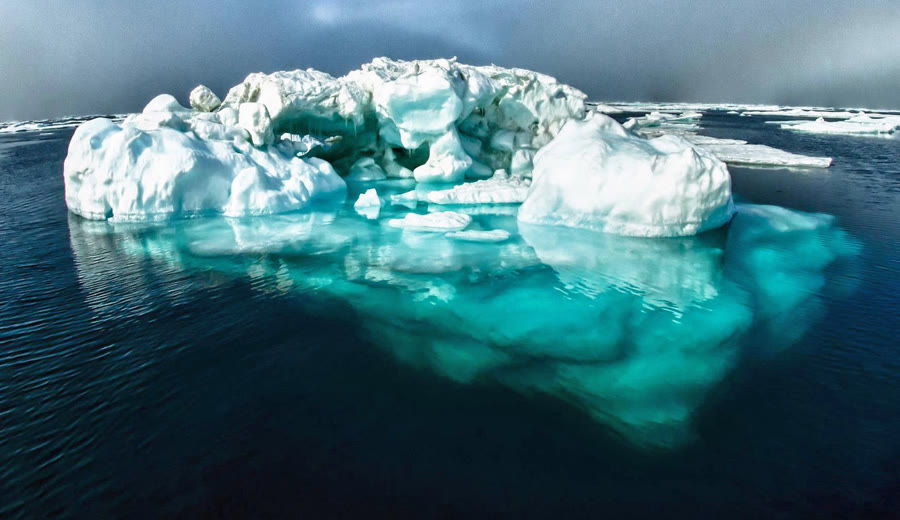
\includegraphics[width=0.66\linewidth]{images/book2/g11-noaa-iceberg.jpg}

{\small An iceberg seen from just above the water: the ice under the surface,
which shows through the clear sea, is far bigger than the part in the air.
Photograph: NOAA (public domain).}
\end{omfigure}
% ledger: photo:g11-iceberg

\section{Two ways to layer the Earth}

The crust, the mantle and the core are layers of different
\emph{materials}: the crust is made of rocks rich in silicon, aluminium and
oxygen, the mantle of a denser rock, the core of metal. But the outer part of
the Earth can also be divided by how its rock \emph{behaves} when forces act
on it for a very long time.

\begin{definition}[Lithosphere; asthenosphere]\label{def:g11:lithosphere-asthenosphere:lithosphere}
The \emph{lithosphere}\index{lithosphere} is the rigid outer shell of the
Earth: the crust and the uppermost, coldest part of the mantle, which together
break into the tectonic plates and do not flow. The
\emph{asthenosphere}\index{asthenosphere} is the layer of the mantle beneath
the lithosphere, hotter and weaker, which flows
slowly over long spans of time, like a very stiff paste.
\end{definition}

The boundary between the two lies about 70 to \qty{100}{km} down under the
oceans and most continents, and deeper under the oldest parts of the
continents; across the United States, for instance, the \omterm{def:g11:lithosphere-asthenosphere:lithosphere}{lithosphere} is from
about \qty{40}{km} thick in the west to more than \qty{200}{km} thick in the
middle of the continent. The base of the \omterm{def:g11:lithosphere-asthenosphere:lithosphere}{lithosphere} is not the \omterm{def:g11:seismic-structure:moho}{Moho}: most of
the \omterm{def:g11:lithosphere-asthenosphere:lithosphere}{lithosphere} is mantle rock.
% ledger: rs09:lab, fischer:lab, porter:lab, usgs:lithosphere-80km (Book 1 row)

\begin{omfigure}
\begin{tikzpicture}[x=1cm, y=-0.0125cm, font=\footnotesize]
% depths to scale: crust 41 km (cm95:crust), lithosphere 100 km (rs09:lab), 0-400 km
  \shade[top color=omLithPeridotite!70, bottom color=omLithPeridotite!25] (5,100) rectangle (8,400);
  \fill[omLithGranite!55] (0,0) rectangle (3,41);
  \fill[omLithPeridotite!55] (0,41) rectangle (3,400);
  \fill[black!25] (5,0) rectangle (8,100);
  \draw (0,0) rectangle (3,400);
  \draw (5,0) -- (5,400) (8,0) -- (8,400) (5,0) -- (8,0);
  \draw[line width=0.8pt] (0,41) -- (3,41);
  \draw[line width=0.8pt, densely dashed] (5,100) -- (8,100);
  \draw[densely dotted, black!60] (3,41) -- (5,41);
  \node at (1.5,20) {crust};
  \node[align=center] at (1.5,220) {mantle};
  \node[align=center] at (6.5,50) {lithosphere\\rigid};
  \node[align=center] at (6.5,180) {asthenosphere\\weak, flows slowly};
  \node[align=center, text=black!70] at (6.5,340) {deeper mantle};
  \node[anchor=south, font=\small] at (1.5,0) {by material};
  \node[anchor=south, font=\small] at (6.5,0) {by behaviour};
  \foreach \d in {0,100,200,300,400} {\draw (-0.1,\d) -- (0,\d); \node[anchor=east] at (-0.1,\d) {\d};}
  \node[anchor=east, rotate=90, anchor=south] at (-0.9,200) {depth (\unit{km})};
  \node[anchor=south, font=\scriptsize, align=center] at (4,41) {Moho\\(\qty{41}{km})};
  \node[anchor=west, align=left] at (8.15,100) {base of the\\lithosphere\\(about \qty{100}{km})};
\end{tikzpicture}

{\small The upper \qty{400}{km} of the Earth under a continent, to scale.
Left: the layers by material. Right: the layers by behaviour. The rigid
\omterm{def:g11:lithosphere-asthenosphere:lithosphere}{lithosphere} contains the whole crust and the top of the mantle; the
\omterm{def:g11:lithosphere-asthenosphere:lithosphere}{asthenosphere} has no sharp lower limit.}
\end{omfigure}

\section{The low-velocity zone}

Seismic waves show the \omterm{def:g11:lithosphere-asthenosphere:lithosphere}{asthenosphere}. Almost everywhere in the Earth, seismic
speeds increase with depth, because the rock is more and more squeezed. Under
the \omterm{def:g11:lithosphere-asthenosphere:lithosphere}{lithosphere} the opposite happens.

\begin{definition}[Low-velocity zone]\label{def:g11:lithosphere-asthenosphere:lvz}
The \emph{low-velocity zone}\index{low-velocity zone} is the layer of the
upper mantle, below the \omterm{def:g11:lithosphere-asthenosphere:lithosphere}{lithosphere}, in which seismic waves travel more slowly
than in the rock above and below it.
\end{definition}

In the \omterm{def:g11:seismic-structure:reference-model}{reference Earth model}, the S speed falls slowly from the \omterm{def:g11:seismic-structure:moho}{Moho} down to
\qty{220}{km}, then jumps up. Seismic studies all over the world find a
sharp drop of speed somewhere between 70 and \qty{100}{km}: the top of the
\omterm{def:g11:lithosphere-asthenosphere:lithosphere}{asthenosphere}. The rock there is hot enough to be close to melting, and may
contain a very little melt; it may also hold more water than the rock above.
Rock close to melting is weak: it slows seismic waves, and it can flow.
% ledger: data:prem, rs09:lab, fischer:lab, porter:lab

\begin{omfigure}
\begin{tikzpicture}
\begin{axis}[omrecord, omdepth, width=0.6\linewidth, height=6.0cm, xmin=3.0, xmax=5.0, ymin=0, ymax=400,
  xlabel={S speed (\unit{km/s})}, ylabel={depth (\unit{km})}, xtick={3.0,3.5,...,5.0},
  xticklabel style={/pgf/number format/fixed, /pgf/number format/precision=1},
  tick label style={font=\small}, label style={font=\small}]
% computed in figdata/grade-11/prem_profiles.py (part upper); ledger: data:prem
\fill[black!10] (axis cs:3.0,80) rectangle (axis cs:5.0,220);
\addplot[omProp, line width=0.9pt] table[x=vs, y=depth] {figdata/out/grade-11-prem_profiles-upper.dat};
\node[font=\scriptsize, anchor=west, align=left] at (axis cs:3.1,150) {low-velocity\\zone};
\node[font=\scriptsize, anchor=west] at (axis cs:3.95,12) {crust};
\end{axis}
\end{tikzpicture}

{\small The S speed in the upper \qty{400}{km} of the \omterm{def:g11:seismic-structure:reference-model}{reference Earth model}.
Below the crust, the speed decreases slowly with depth down to
\qty{220}{km} (shaded from \qty{80}{km}), then increases again with sudden
steps.}
\end{omfigure}

\section{The geotherm}

\begin{definition}[Geotherm; geothermal gradient]\label{def:g11:lithosphere-asthenosphere:geotherm}
A \emph{geotherm}\index{geotherm} is the curve of temperature against depth
beneath a place. The \emph{geothermal gradient}\index{geothermal gradient} is
the rise of temperature per unit of depth, in degrees per kilometre.
\end{definition}

Boreholes measure the \omterm{def:g11:lithosphere-asthenosphere:geotherm}{geotherm} only in the first few kilometres, where the
temperature rises by 25 to \qty{30}{\celsius} per kilometre (Book 1,
grade 6). Deeper, it is computed from the heat that flows out through the
surface and from the properties of the rocks; \cref{ch:g12:internal-heat}
shows where that heat comes from. Two facts shape the result. Part of the
heat is made inside the upper crust itself, so the gradient is steepest near
the surface and smaller below the crust. And in the \omterm{def:g11:lithosphere-asthenosphere:lithosphere}{asthenosphere}, which
flows, the slow motion of the rock carries the heat and evens out the
temperature: it rises only about \qty{0.45}{\celsius} per kilometre. The
base of the \omterm{def:g11:lithosphere-asthenosphere:lithosphere}{lithosphere} is placed where the steep \omterm{def:g11:lithosphere-asthenosphere:geotherm}{geotherm} of the \omterm{def:g11:lithosphere-asthenosphere:lithosphere}{lithosphere}
meets the gentle one of the \omterm{def:g11:lithosphere-asthenosphere:lithosphere}{asthenosphere}, at about \qty{1300}{\celsius}.
% ledger: usgs:gradient-29 (Book 1 row), b2dd10:continents, b2roy:provinces, roy:conductivity,
% katsura10:adiabat, porter:lab

\begin{omfigure}
\begin{tikzpicture}
\begin{axis}[omrecord, omdepth, width=0.7\linewidth, height=6.4cm, xmin=0, xmax=2000, ymin=0, ymax=300,
  xlabel={temperature (\unit{\celsius})}, ylabel={depth (\unit{km})}, xtick={0,500,...,2000},
  tick label style={font=\small}, label style={font=\small}]
% computed in figdata/grade-11/geotherm_solidus.py; ledger: b2dd10:continents, b2roy:provinces,
% roy:conductivity, porter:lab, katsura10:adiabat, hirschmann:solidus, data:prem
\fill[black!8] (axis cs:0,99.7) rectangle (axis cs:2000,300);
\addplot[omDef, line width=1.0pt] table[x=t_geotherm, y=depth_km] {figdata/out/grade-11-geotherm_solidus-geotherm.dat};
\addplot[omDef, densely dashed, restrict y to domain=99:300] table[x=t_cond, y=depth_km] {figdata/out/grade-11-geotherm_solidus-geotherm.dat};
\addplot[omProp, line width=1.0pt] table[x=t_solidus, y=depth_km] {figdata/out/grade-11-geotherm_solidus-geotherm.dat};
\draw[black!60] (axis cs:0,99.7) -- (axis cs:2000,99.7);
\node[font=\scriptsize, anchor=south west] at (axis cs:20,99.7) {base of the lithosphere};
\node[font=\scriptsize, anchor=north west] at (axis cs:20,102) {asthenosphere};
\node[font=\scriptsize, text=omDef, anchor=north west] at (axis cs:480,6) {geotherm};
\node[font=\scriptsize, text=omProp, anchor=west] at (axis cs:1300,22) {melting begins};
\end{axis}
\end{tikzpicture}

{\small A model \omterm{def:g11:lithosphere-asthenosphere:geotherm}{geotherm} under a continent (blue) and the temperature at
which mantle rock (peridotite, without water) begins to melt (orange). The
\omterm{def:g11:lithosphere-asthenosphere:geotherm}{geotherm} is computed from the mean heat flow of the continents and measured
rock properties; in the \omterm{def:g11:lithosphere-asthenosphere:lithosphere}{asthenosphere} (grey) it rises slowly. The dashed line shows
how the \omterm{def:g11:lithosphere-asthenosphere:lithosphere}{lithosphere}'s steeper rise would continue. The two curves come
closest, about \qty{140}{\celsius} apart, near the base of the \omterm{def:g11:lithosphere-asthenosphere:lithosphere}{lithosphere}.}
\end{omfigure}
% values: lab_km 99.7, t_lab_c 1345, closest_gap_c 144 (figdata/grade-11/geotherm_solidus.py)

The melting temperature of the mantle rock rises with depth, because the
rock is more and more squeezed (Book 1, grade 6): about \qty{1120}{\celsius}
at the surface, nearly \qty{1500}{\celsius} at \qty{100}{km}. In the model,
the \omterm{def:g11:lithosphere-asthenosphere:geotherm}{geotherm} comes closest to it just below the \omterm{def:g11:lithosphere-asthenosphere:lithosphere}{lithosphere}, about
\qty{140}{\celsius} short of it. A little water, or a slightly hotter
mantle, closes the gap: in the west of the United States, where the
\omterm{def:g11:lithosphere-asthenosphere:lithosphere}{lithosphere} is thin, a little of the mantle beneath it is partly molten.
% ledger: hirschmann:solidus, porter:lab; computed in figdata/grade-11/geotherm_solidus.py
% (solidus0_c 1120.7, solidus100_c 1489, closest_gap_c 144)

\section{Isostasy}

\subsection{Floating on a solid}

Over the few seconds of an earthquake wave, the \omterm{def:g11:lithosphere-asthenosphere:lithosphere}{asthenosphere} is a solid. Over
long spans of time, it flows. A load placed on the \omterm{def:g11:lithosphere-asthenosphere:lithosphere}{lithosphere} --- a mountain
range, an ice sheet --- slowly pushes the \omterm{def:g11:lithosphere-asthenosphere:lithosphere}{asthenosphere} aside until the load
floats, like a block of wood on water.

\begin{definition}[Isostasy; compensation depth]\label{def:g11:lithosphere-asthenosphere:isostasy}
\emph{Isostasy}\index{isostasy} is the balance in which the outer layers of
the Earth float on the \omterm{def:g11:lithosphere-asthenosphere:lithosphere}{asthenosphere}: at a depth in the mantle called the
\emph{compensation depth}\index{compensation depth}, every column of rock of
the same cross-section, from the surface down to that depth, has the same
weight, whatever the relief above it.
\end{definition}

\begin{omfigure}
\begin{tikzpicture}[x=1cm, y=1cm, font=\footnotesize, >={Stealth[length=4pt]}]
% not to scale
  \fill[omSea!50] (6,0) rectangle (8.6,-0.9);
  \fill[omLithPeridotite!45] (0,-5.2) rectangle (2.6,-6.6);
  \fill[omLithGranite!55] (0,2.0) -- (2.6,2.0) -- (2.6,-5.2) -- (0,-5.2) -- cycle;
  \fill[omLithGranite!55] (2.6,0) rectangle (6,-3.0);
  \fill[omLithGranite!55] (6,-0.9) rectangle (8.6,-1.6); % same fill: one crustal density in Airy's model
  \fill[omLithPeridotite!45] (2.6,-3.0) rectangle (6,-6.6);
  \fill[omLithPeridotite!45] (6,-1.6) rectangle (8.6,-6.6);
  \draw (0,2.0) -- (2.6,2.0) -- (2.6,0) -- (6,0);
  \draw (6,0) -- (8.6,0);
  \draw[line width=0.8pt] (0,-5.2) -- (2.6,-5.2) -- (2.6,-3.0) -- (6,-3.0) -- (6,-1.6) -- (8.6,-1.6);
  \draw[densely dashed, line width=0.8pt] (0,-6.2) -- (8.6,-6.2);
  \node[anchor=north east] at (8.6,-6.6) {compensation depth};
  \draw[black!50, densely dotted] (-0.2,0) -- (0,0);
  \node[anchor=east] at (-0.2,0) {sea level};
  \node at (1.3,-1.6) {crust};
  \node at (4.3,-1.5) {crust};
  \node at (7.3,-0.45) {ocean};
  \node at (7.3,-1.25) {crust};
  \node at (4.3,-4.8) {mantle};
  \node[anchor=south] at (1.3,2.0) {mountain range};
  \node[anchor=south] at (4.3,0) {lowland};
  \draw[<->] (2.75,0) -- (2.75,2.0); \node[anchor=west] at (2.8,1.0) {$h$};
  \draw[<->] (2.75,-3.0) -- (2.75,-5.2); \node[anchor=west] at (2.8,-4.1) {root $r$};
  \draw[<->] (5.85,0) -- (5.85,-3.0); \node[anchor=east] at (5.8,-1.0) {$T$};
\end{tikzpicture}

{\small Airy's model of \omterm{def:g11:lithosphere-asthenosphere:isostasy}{isostasy} (not to scale). The crust is everywhere of
the same density; where it stands high, it is thick and has a root that
reaches deep into the denser mantle. Under the ocean, the crust is thin. All
three columns weigh the same down to the \omterm{def:g11:lithosphere-asthenosphere:isostasy}{compensation depth}.}
\end{omfigure}

\subsection{The root of a mountain range}

\begin{proposition}[Airy isostasy]\label{prop:g11:lithosphere-asthenosphere:airy}
Let the crust have a uniform density $\rho_c$, and the mantle beneath it a
density $\rho_m > \rho_c$. If a region stands a height $h$ above another one
and both are in isostatic balance, its crust is thicker by
\[
  \Delta H = h\,\frac{\rho_m}{\rho_m - \rho_c},
\]
of which $h$ stands above the other region and a root
$r = h\,\rho_c/(\rho_m - \rho_c)$ reaches below its crust.\index{Airy isostasy}
\end{proposition}

\begin{proof}
Take two columns of the same area $S$, the lowland with a crust of thickness
$T$ and the range, whose crust stands $h$ higher and reaches $r$ deeper, so
that its thickness is $T + h + r$. Down to a \omterm{def:g11:lithosphere-asthenosphere:isostasy}{compensation depth} below both
\omterm{def:g11:seismic-structure:moho}{Mohos}, the range column has $h + r$ more crust; the lowland column has,
instead, mantle over the thickness $r$. With $g$ the acceleration of gravity,
the two weights are equal when
\[
  \rho_c\,(h + r)\,S\,g = \rho_m\,r\,S\,g,
  \qquad\text{that is}\qquad
  r = h\,\frac{\rho_c}{\rho_m - \rho_c}.
\]
The crust is thicker by $h + r = h\,\bigl(1 + \rho_c/(\rho_m - \rho_c)\bigr)
= h\,\rho_m/(\rho_m - \rho_c)$.
\end{proof}

With the mean density of the continental crust, $\rho_c =
\qty{2830}{kg/m^3}$, and that of the mantle just below the \omterm{def:g11:seismic-structure:moho}{Moho}, $\rho_m =
\qty{3380}{kg/m^3}$, the root is $2830/550 \approx 5.1$ times the height,
and the crust is thicker by about $6.1$ times the height: a range
\qty{3}{km} above its surroundings has a root of about \qty{15}{km}.
% ledger: cm95:crust, data:prem (rho 3.38 below the Moho)

\begin{method}[Computing a root]\label{met:g11:lithosphere-asthenosphere:root}
\begin{enumerate}
  \item Find the height $h$ of the region above a reference region whose crust
        thickness is known.
  \item Compute $\rho_m/(\rho_m - \rho_c)$ with the densities of crust and
        mantle.
  \item The crust is thicker than the reference crust by $h\,\rho_m/(\rho_m -
        \rho_c)$; the root alone is that minus $h$.
\end{enumerate}
\end{method}

\begin{example}[A plateau \qty{2}{km} high]\label{ex:g11:lithosphere-asthenosphere:plateau}
A plateau stands \qty{2}{km} above a lowland whose crust is \qty{37}{km}
thick. Its crust is thicker by $2 \times 3380/550 \approx \qty{12.3}{km}$:
about \qty{49}{km} in all, with a root of about \qty{10}{km}.
\end{example}

\subsection{Why the continents stand high}

\begin{definition}[Hypsometric curve]\label{def:g11:lithosphere-asthenosphere:hypsometry}
The \emph{hypsometric curve}\index{hypsometric curve} of the Earth gives, for
each elevation, the fraction of the Earth's surface that lies higher than it.
Its slope shows how much of the surface lies at each elevation.
\end{definition}

If the surface had been shaped by chance, most of it would lie near one
average level. It does not.

\begin{proposition}[Two levels]\label{prop:g11:lithosphere-asthenosphere:two-levels}
The elevations of the Earth's surface cluster around two levels: one within
a few hundred metres of sea level, on the continents, and one about 4 to
\qty{5}{km} below sea level, on the deep ocean floor. Land covers \qty{29}{\percent}
of the surface; more than half of the surface lies deeper than \qty{3}{km}
below sea level, and only \qty{3}{\percent} rises higher than \qty{2}{km}.
\end{proposition}
% computed in figdata/grade-11/hypsometry.py from ETOPO1 (land_fraction 0.290,
% share_below_3000_pct 53.4, share_above_2000_pct 3.1; modes at +250 and -4250 m); ledger: data:etopo1

\begin{omfigure}
\begin{tikzpicture}
\begin{axis}[omrecord, width=0.86\linewidth, height=5.4cm, xmin=-11000, xmax=9000, ymin=0, ymax=18,
  xlabel={elevation (\unit{m}; negative: below sea level)}, ylabel={share of the surface (\unit{\percent})},
  xtick={-10000,-8000,...,8000}, scaled x ticks=false, xticklabel style={/pgf/number format/1000 sep={\,}, font=\scriptsize},
  tick label style={font=\small}, label style={font=\small}, clip=false]
% computed in figdata/grade-11/hypsometry.py; ledger: data:etopo1
\addplot[ybar interval, fill=omSea!70, draw=black!50, restrict expr to domain={\thisrow{land}}{0:0}] table[x=lo, y=share_pct] {figdata/out/grade-11-hypsometry-bins.dat};
\addplot[ybar interval, fill=omHypsLandC, draw=black!50, restrict expr to domain={\thisrow{land}}{1:1}] table[x=lo, y=share_pct] {figdata/out/grade-11-hypsometry-bins.dat};
\draw[black!60, densely dotted] (axis cs:0,0) -- (axis cs:0,18);
\node[font=\scriptsize, anchor=south west] at (axis cs:600,15.5) {continents};
\node[font=\scriptsize, anchor=south] at (axis cs:-4250,12.2) {deep ocean floor};
\end{axis}
\end{tikzpicture}

{\small Share of the Earth's surface in each band of \qty{500}{m} of
elevation (from ETOPO1, at one degree; over Antarctica and Greenland, the
top of the ice). The two peaks are the continents and the deep ocean floor.}
\end{omfigure}

\omterm{def:g11:lithosphere-asthenosphere:isostasy}{Isostasy} explains the two levels. The continents are made of a thick crust,
about \qty{41}{km} on average, of light rock; the ocean floor of a thin crust
of denser rock, only about \qty{5}{km} thick. Both float on the
\omterm{def:g11:lithosphere-asthenosphere:lithosphere}{asthenosphere}: the thick, light continental crust floats high, the thin, dense
oceanic crust low, and the oceans fill the low ground.
% ledger: cm95:crust, usgs:crust-thickness (Book 1 row)

\section{A flexible lid}

\omterm{def:g11:lithosphere-asthenosphere:isostasy}{Isostasy} needs the \omterm{def:g11:lithosphere-asthenosphere:lithosphere}{asthenosphere} to flow. The \omterm{def:g11:lithosphere-asthenosphere:lithosphere}{lithosphere} above it does not
flow; it bends. A load narrower than the thickness of the \omterm{def:g11:lithosphere-asthenosphere:lithosphere}{lithosphere}, such
as a single volcanic island, is carried by the stiffness of the plate, like a
weight on a plank, and the plate sags around it. A load much wider than that
thickness, such as a whole mountain range or an ice sheet, sinks until it
floats. When the load is removed, the \omterm{def:g11:lithosphere-asthenosphere:lithosphere}{lithosphere} slowly rises again
(\cref{ch:g12:destruction-of-mountains}).

\section{Exercises}

\begin{exercise}[$\star$]\label{exo:g11:lithosphere-asthenosphere:1}
Define the \omterm{def:g11:lithosphere-asthenosphere:lithosphere}{lithosphere} and the \omterm{def:g11:lithosphere-asthenosphere:lithosphere}{asthenosphere}. Which of the following belong
to the \omterm{def:g11:lithosphere-asthenosphere:lithosphere}{lithosphere}: the oceanic crust, the continental crust, the uppermost
mantle, the outer core?
\end{exercise}

\begin{exercise}[$\star$]\label{exo:g11:lithosphere-asthenosphere:2}
An iceberg of density \qty{910}{kg/m^3} floats in sea water of density
\qty{1025}{kg/m^3}. What fraction of its volume lies under water? If an
iceberg with vertical sides stands \qty{20}{m} above the water, what is its
total height?
\end{exercise}

\begin{exercise}[$\star$]\label{exo:g11:lithosphere-asthenosphere:3}
The ground is at \qty{15}{\celsius} and the \omterm{def:g11:lithosphere-asthenosphere:geotherm}{geothermal gradient} is
\qty{26}{\celsius} per kilometre. What is the temperature at the bottom of a
borehole \qty{3}{km} deep? Why can the same gradient not be used down to
\qty{100}{km}?
\end{exercise}

\begin{exercise}[$\star$]\label{exo:g11:lithosphere-asthenosphere:4}
From the figure of the elevations of the Earth's surface, give the two most
common elevation bands and the share of the surface in each.
\end{exercise}

\begin{exercise}[$\star$]\label{exo:g11:lithosphere-asthenosphere:5}
With the formula $T = -5.104\,P^2 + 132.899\,P + 1120.661$ (temperature in
\unit{\celsius}, pressure $P$ in gigapascals), compute the temperature at
which dry mantle rock begins to melt at the surface ($P = 0$) and at
\qty{3}{GPa}, about \qty{95}{km} down.
\end{exercise}

\begin{exercise}[$\star\star$]\label{exo:g11:lithosphere-asthenosphere:6}
On the figure of the model \omterm{def:g11:lithosphere-asthenosphere:geotherm}{geotherm}, read the temperature at 50, 150 and
\qty{250}{km}. In which layer, \omterm{def:g11:lithosphere-asthenosphere:lithosphere}{lithosphere} or \omterm{def:g11:lithosphere-asthenosphere:lithosphere}{asthenosphere}, is each depth?
Between which two of these depths does the temperature rise most?
\end{exercise}

\begin{exercise}[$\star\star$]\label{exo:g11:lithosphere-asthenosphere:7}
A mountain range stands \qty{3}{km} above a lowland; take $\rho_c =
\qty{2830}{kg/m^3}$ and $\rho_m = \qty{3380}{kg/m^3}$. Compute its root and
the extra thickness of its crust.
\end{exercise}

\begin{exercise}[$\star\star$]\label{exo:g11:lithosphere-asthenosphere:8}
A region has a crust \qty{55}{km} thick. With the densities of
\cref{exo:g11:lithosphere-asthenosphere:7}, how high does it stand above a
region whose crust is \qty{41.1}{km} thick?
\end{exercise}

\begin{exercise}[$\star\star$]\label{exo:g11:lithosphere-asthenosphere:9}
In the reference model, the S speed is \qty{4.470}{km/s} at \qty{80}{km},
\qty{4.419}{km/s} just above \qty{220}{km} and \qty{4.644}{km/s} just below.
Compute, in per cent, the decrease between 80 and \qty{220}{km} and the jump
at \qty{220}{km}. Why is a decrease of speed with depth surprising?
\end{exercise}

\begin{exercise}[$\star\star$]\label{exo:g11:lithosphere-asthenosphere:10}
In the model \omterm{def:g11:lithosphere-asthenosphere:geotherm}{geotherm}, the temperature is \qty{610}{\celsius} at the \omterm{def:g11:seismic-structure:moho}{Moho},
\qty{40}{km} down, and \qty{1345}{\celsius} at the base of the \omterm{def:g11:lithosphere-asthenosphere:lithosphere}{lithosphere},
\qty{100}{km} down. (1) Compute the mean gradient between the two. (2)
Compare with the gradient at the surface, \qty{26}{\celsius} per kilometre,
and explain the difference.
\end{exercise}

\begin{exercise}[$\star\star$]\label{exo:g11:lithosphere-asthenosphere:11}
In the \omterm{def:g11:lithosphere-asthenosphere:lithosphere}{asthenosphere} the temperature is taken as $1300 + 0.45\,z$ (in
\unit{\celsius}, $z$ in kilometres). Compute it at 200 and \qty{400}{km}. By
how much does it rise between the two? Compare with the rise through the
first \qty{100}{km}, from \qty{15}{\celsius} at the surface to
\qty{1345}{\celsius} at the base of the \omterm{def:g11:lithosphere-asthenosphere:lithosphere}{lithosphere}.
\end{exercise}

\begin{exercise}[$\star\star\star$]\label{exo:g11:lithosphere-asthenosphere:12}
Below the upper crust, the model \omterm{def:g11:lithosphere-asthenosphere:geotherm}{geotherm} is close to $T \approx 118 +
G\,z$ (in \unit{\celsius}, $z$ in kilometres), where the gradient $G$
depends on the heat coming from deeper down. (1) For $G =
\qty{12.3}{\celsius}$ per kilometre, as computed for the east of the United
States, find the depth at which it meets $1300 + 0.45\,z$. (2) Do the same
for $G = \qty{21.5}{\celsius}$ per kilometre, as computed for the Basin and
Range province of the west. (3) Compare with the measured thicknesses, from about
\qty{40}{km} in the west to more than \qty{200}{km} in the middle of the
continent.
\end{exercise}

\begin{exercise}[$\star\star\star$]\label{exo:g11:lithosphere-asthenosphere:13}
(1) Show that, in Airy's model, a region whose crust is $\Delta H$ thicker
than a reference region stands higher by $\Delta H\,(\rho_m - \rho_c)/\rho_m$.
(2) What fraction of any extra thickness of crust appears as height? (3)
Compare with the fraction of an iceberg that stands above the water.
\end{exercise}

\begin{exercise}[$\star\star\star$]\label{exo:g11:lithosphere-asthenosphere:14}
At \qty{100}{km} the dry mantle rock begins to melt at \qty{1489}{\celsius},
and the model \omterm{def:g11:lithosphere-asthenosphere:geotherm}{geotherm} is at \qty{1345}{\celsius}. (1) By how many degrees
would water have to lower the melting temperature for the rock to start
melting there? (2) Why would even a very small fraction of melt make the
rock weak and slow down seismic waves?
\end{exercise}

\begin{exercise}[$\star\star\star$]\label{exo:g11:lithosphere-asthenosphere:15}
Only \qty{3}{\percent} of the Earth's surface rises above \qty{2}{km}, while
\qty{53}{\percent} lies more than \qty{3}{km} below sea level. (1) If all the
land were planed flat and its rock dumped into the oceans, would the surface
end up near sea level? Use \omterm{def:g11:lithosphere-asthenosphere:isostasy}{isostasy} to explain your answer. (2) What does
the existence of two levels tell us about the crust?
\end{exercise}

\section{Problem: Why Tibet Stands Five Kilometres High}

\begin{problem}[{Weekend problem --- weighing a plateau}]
\label{pb:g11:lithosphere-asthenosphere:1}
% values computed in figdata/grade-11/hypsometry.py (tibet_mean_m 5015, qaidam_mean_m 3230,
% mean_land_no_antarctica_m 674); ledger: data:etopo1, cm95:crust, data:prem, karplus:tibet-moho
The Tibetan plateau is the largest high region on Earth. Between latitudes
\ang{31} and \ang{35} North and longitudes \ang{80} and \ang{95} East, its
mean elevation is \qty{5010}{m}; the mean elevation of all the land outside
Antarctica is \qty{670}{m}. The continental crust is \qty{41.1}{km} thick on
average and has a mean density $\rho_c = \qty{2830}{kg/m^3}$; the mantle just
below the \omterm{def:g11:seismic-structure:moho}{Moho} has the density $\rho_m = \qty{3380}{kg/m^3}$.

\medskip
\noindent\textbf{Part I --- The plateau and an average continent.}
\begin{enumerate}
  \item How much higher than the average continent does the plateau stand?
  \item By what percentage is the crust less dense than the mantle beneath it?
  \item A block of crust floating freely on mantle rock would sink until what
        fraction of its thickness lay below the mantle's surface? Compare with
        the iceberg ($910$ in $1025$).
  \item The mantle is solid. Over which spans of time does it behave as a
        solid, and over which can it behave like the water around an
        iceberg?
  \item Why must the \omterm{def:g11:lithosphere-asthenosphere:isostasy}{compensation depth} be chosen below the \omterm{def:g11:seismic-structure:moho}{Moho} of both
        columns?
\end{enumerate}

\medskip
\noindent\textbf{Part II --- Airy's balance for two columns.}
\begin{enumerate}[resume]
  \item Draw the two columns, the average continent and the plateau, from
        their surfaces down to a depth of \qty{70}{km} below sea level, with
        the plateau's crust thicker by $\Delta H$.
  \item Write that the two columns weigh the same, and deduce $\Delta H$ in
        terms of the height difference $h$ and of the densities.
  \item Compute $\rho_m/(\rho_m - \rho_c)$.
  \item Compute the root of the plateau below the \omterm{def:g11:seismic-structure:moho}{Moho} of the average
        continent.
  \item How deep below sea level is the \omterm{def:g11:seismic-structure:moho}{Moho} of the average continent, and
        how deep is that of the plateau?
\end{enumerate}

\medskip
\noindent\textbf{Part III --- The thickness of the crust.}
\begin{enumerate}[resume]
  \item Compute the thickness of the crust under the plateau.
  \item Check the balance: compute, for each column, the mass of rock above
        a square metre down to \qty{70}{km} below sea level, in tonnes.
  \item How thick would the crust be under a lowland at sea level?
  \item How many times thicker than the average continental crust is the
        crust under Tibet?
  \item If the mantle were a little lighter, $\rho_m = \qty{3300}{kg/m^3}$,
        what thickness would the model give? Is the result very sensitive to
        the densities?
\end{enumerate}

\medskip
\noindent\textbf{Part IV --- Comparison with the seismic measurements.}
\begin{enumerate}[resume]
  \item Seismic waves converted at the \omterm{def:g11:seismic-structure:moho}{Moho} place it about \qty{70}{km} down
        beneath northern Tibet. Compare with question~11.
  \item Just north of the plateau, the Qaidam basin stands at a mean
        elevation of \qty{3230}{m}, and its \omterm{def:g11:seismic-structure:moho}{Moho} lies about \qty{50}{km}
        down. What crust thickness does Airy's model predict there?
  \item The Qaidam basin is filled with several kilometres of sediments,
        lighter than average crust. Does that make the real crust thinner or
        thicker than the model's? Explain.
  \item What property of the \omterm{def:g11:lithosphere-asthenosphere:lithosphere}{asthenosphere} makes such a balance possible?
  \item Conclude: how thick is the crust under Tibet, and why does the
        plateau stand five kilometres high?
\end{enumerate}
\end{problem}
